\section{Case Study JAK-STAT}
Let us study the hidden input observation problem for a linearised version of the 
JAK-STAT loop. Consider the linear dynamic system
\begin{equation}
	\dot{x} = A x + B u \tab{,} x(0)=x_0 \tab{,} y = Cx
\end{equation}
with
\begin{equation}
	A = \begin{pmatrix}
	-\alpha_1 & 0 & 0 & \beta_4 \\ \beta_1 & -\alpha_2 & 0 & 0 \\
	0 & \beta_2 & -\alpha_3 & 0 \\ 0 & 0 & \beta_3 & -\alpha_4
	\end{pmatrix} \tab{,} 
	B = \begin{pmatrix}
	1 & 0 \\ 0 & 1
	\end{pmatrix} \tab{,}
	C = \begin{pmatrix}
	c_1 & c_1 & c_1 & 0 \\ 0 & c_2 & c_2 & 0
	\end{pmatrix} \quad .
\end{equation}
Since the known inputs have no effect on the hidden input observability, let us set 
$u \equiv 0$. Furthermore we assume that all parameters are nonzero and ignore special 
cases in which parameters annihilate, e.g. we assume $\beta_1-\alpha_1 = 0$ does not 
happen. An illustration can be found in figure \ref{fig:network_graph}.

\begin{figure}[h]
	\centering
	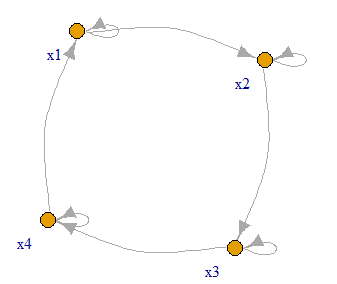
\includegraphics[scale=0.7]{bilder/JAKSTAT_network_graph.png}
	\caption{The network graph of the linearized JAK-STAT model.}
	\label{fig:network_graph}
\end{figure}

\clearpage
\subsection*{Check for HIO via reduced matrices}
We will use the theorem with reduced matrices to check whether this system 
is hidden input observable or not. Let us recap the theorem and the corresponding 
algorithm. 
\begin{remark}{Reduced Matrices}{}
	\begin{enumerate}
		\item Choose an injective $4 \times m$ matrix $D$ where $m$ is the number of hidden 
		inputs. 
		\item Compute $CD,CAD,CA^2D,\ldots$ up to an appropriate power of 
		$A$. In this particular case the first power $CAD$ suffices. 
		\item Memorise the locations of all nonzero columns of $CD$ in an index set 
		$\mathcal{I}_0$. 
		\item Reduce $CD$ to the columns in $\mathcal{I}_0$, i.e. nonzero columns, to get 
		$(CD)^*$.
		\item Memorise the locations of all nonzero columns of $CAD$ in $\mathcal{I}_1$.
		\item Append the $i$-th column of $CAD$ to $(CD)^*$ if $i\in\mathcal{I}_1\backslash 
		\mathcal{I}_0$ to get $(CAD)^*$.
	\end{enumerate}
	If each reduced matrix $(CA^kD)^*$ is injective and if there is an integer $K$ such 
	that $(CA^KD^*)$ has rank $m$, then the system is hidden input observable.
\end{remark}
To fulfil the rank condition it is necessary to have at least as many outputs as inputs. In 
this case $m\leq 2$. Let us analyse the six input matrices 
\begin{align*}
D_{12} &= \begin{pmatrix} 1 & 0 \\ 0 & 1 \\ 0 & 0 \\ 0 & 0 \end{pmatrix} \tab{,}
D_{13} = \begin{pmatrix} 1 & 0 \\ 0 & 0 \\ 0 & 1 \\ 0 & 0 \end{pmatrix} \tab{,}
D_{14} = \begin{pmatrix} 1 & 0 \\ 0 & 0 \\ 0 & 0 \\ 0 & 1 \end{pmatrix} \tab{,} \\
D_{23} &= \begin{pmatrix} 0 & 0 \\ 1 & 0 \\ 0 & 1 \\ 0 & 0 \end{pmatrix} \tab{,}
D_{24} = \begin{pmatrix} 0 & 0 \\ 1 & 0 \\ 0 & 0 \\ 0 & 1 \end{pmatrix} \tab{,}
D_{34} = \begin{pmatrix} 0 & 0 \\ 0 & 0 \\ 1 & 0 \\ 0 & 1 \end{pmatrix} \quad .
\end{align*}
We get
\begin{align*}
CD_{12} &= \begin{pmatrix} c_1 & c_1 \\ 0 & c_2 \end{pmatrix} \tab{,}
CD_{13} = \begin{pmatrix} c_1 & c_1 \\ 0 & c_2  \end{pmatrix} \tab{,}
CD_{14} = \begin{pmatrix} c_1 & 0 \\ 0 & 0      \end{pmatrix} \tab{,} \\
CD_{23} &= \begin{pmatrix} c_1 & c_1 \\ c_2 & c_2 \end{pmatrix} \tab{,}
CD_{24} = \begin{pmatrix} c_1 & 0 \\ c_2 & 0    \end{pmatrix} \tab{,}
CD_{34} = \begin{pmatrix} c_1 & 0 \\ c_2 & 0   \end{pmatrix} \quad .
\end{align*}
When we reduce these matrices to the nonzero columns we can directly see that $D_{12}$ and 
$D_{13}$ lead to hidden input observability. We also see that $CD_{23}=(CD_{23})^*$ is not 
injective. However the reduced matrix algorithm is sufficient but not necessary for hidden 
input observability. We proceed with
\begin{equation*}
CAD_{14} = \begin{pmatrix} c_1(\beta_1-\alpha_1) & c_1 \beta_4 \\ c_2\beta_1 & 
0\end{pmatrix} \tab{,}
CAD_{24} = \begin{pmatrix} c_1(\beta_2-\alpha_2) & c_1 \beta_4 \\ c_2(\beta_2-\alpha_2) & 0 
\end{pmatrix} \tab{,}
CAD_{34} = \begin{pmatrix} -c_1\alpha_3 & c_1\beta_4 \\ -c_2\alpha_3 & 0      \end{pmatrix} 
\end{equation*}
and get
\begin{equation*}
(CAD_{14})^* = \begin{pmatrix} c_1 & c_1 \beta_4 \\ 0 & 0\end{pmatrix} \tab{,}
(CAD_{24})^* = \begin{pmatrix} c_1 & c_1 \beta_4 \\ c_2& 0 
\end{pmatrix} \tab{,}
(CAD_{34})^* = \begin{pmatrix} c_1 & c_1\beta_4 \\ c_2 & 0      \end{pmatrix}  \quad .
\end{equation*}
Therefore $D_{24}$ and $D_{34}$ also lead to hidden input observability.
Note that in this system none of the reduced matrices contains any self-loop factor 
$\alpha_i$.

\clearpage
\subsection*{Simulation}
Choosing a set of numerical values for the parameters of the model and a 
perturbationfunction $P(t)$, we can numerically 
simulate observations using \textsf{R} and the library \textsf{deSolve}. With the 
\textsf{R} implementation of the \textsf{Dynamic-Elastic-Net} 
\textsf{Greedy-Gradient-Method} we 
then analyse the simulated data and try to reconstruct the perturbation. We chose the 
parameter as depicted in table \ref{tab:parameters} and for simplicity $c_1=1$ 
and $c_2=2$ in all simulations.

\begin{table}[h]
	\centering
	\begin{tabular}{ccccccccccc}
	\toprule\midrule
	 & $\alpha_1$	& $\alpha_2$ & $\alpha_3$ & $\alpha_4$ & $\beta_1$ & $\beta_2$ & 
		$\beta_3$  & $\beta_4$ & $x_0$ \\ \midrule
	I & $0.1$&$0.1$&$0.1$&$0.1$ & $0.2$&$0.2$&$0.2$& $0.2$& $(1,0.01,0.01,0.01)$ \\
	II & $0.1$&$0.1$&$0.1$&$0.1$ & $0.2$&$0.2$&$0.2$& $0.8$& $(1,0.01,0.01,0.01)$ \\
	III \\
	\midrule\bottomrule
	\end{tabular}
	\label{tab:parameters}
\end{table}

We choose the observation time interval to be $[0,10]$ and the perturbation function to be 
\begin{equation}
		P(t) = \frac{1}{1+(t-5)^2} \quad ,
\end{equation}	
the graph can be found in figure \ref{fig:perturbation}. \\

\begin{wrapfigure}{r}{8cm}
	\centering
	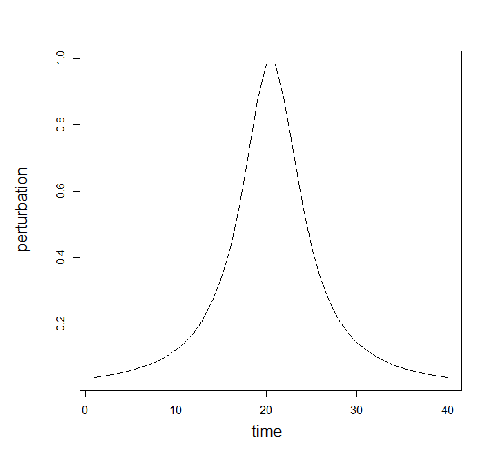
\includegraphics[scale=0.5]{bilder/perturbation.png}
	\caption{The graph of the perturbation $P(t)$.}
	\label{fig:perturbation}
\end{wrapfigure}

We simulated data of a system with perturbation on knot $1$, concrete
	\begin{equation}
	\dot{x}_1 (t) = \sum\limits_{i=1}^4 A_{1i} x_i(t) + P(t) 
	\end{equation}
and gave this data along with the nominal model to the DEN-algorithm. The first step of 
the algorithm is to get a predetermination of all hidden inputs via the gradient-method. 
These results provide the starting point of the greedy-approach. In this case study we only 
calculated the first step since the predetermination of the hidden inputs already shows 
the problem with not observable systems.
	
\clearpage
	\subsubsection*{Observable System}
	We use $D_{13}$ as a hidden input candidate, that is HIO by the reduced-matrix-rank 
	condition. The results for the first two parameter sets can be seen in figures
	\ref{fig:HIO_I} and \ref{fig:HIO_II}. 
	If we compare parameter set I and parameter set II we see, that there is hardly any 
	difference in the predetermination of the hidden inputs.
	
 	\begin{figure}[h]
\centering

	\begin{minipage}{0.45\textwidth}		 
		\centering
		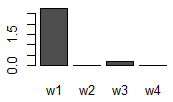
\includegraphics[width=\textwidth]{bilder/D13_I.png}
   		\caption{Results for a observable system with perturbation on knot $1$ 
   		 	and parameter set I.} 
   		 \label{fig:HIO_I}
	\end{minipage}
	%
	\hfill
	%
	\begin{minipage}{0.45\textwidth}
		\vspace{0.0pt} 
		\centering
   		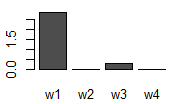
\includegraphics[width=\textwidth]{bilder/D13_II.png}
		\caption{Results for a observable system with perturbation on knot $1$ and 
			parameter set II.} 
		\label{fig:HIO_II}
	\end{minipage}

\end{figure}
		
	
	\subsubsection*{Not Observable System}
	We used $D_{14}$ as a candidate model for hidden inputs. As already seen, this model 
	does not fulfil the reduced-matrix-rank conditions. Indeed, when we compare the results 
	for the parameter sets I and II as depicted in figures \ref{fig:notHIO_I} and 
	\ref{fig:notHIO_II} we see, that a relatively small change in only 
	one parameter is enough to shift the greatest expected hidden input from knot $1$ to 
	knot $4$. 
	
 	\begin{figure}[h]
\centering

	\begin{minipage}{0.45\textwidth}		 
		\centering
		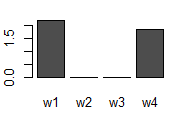
\includegraphics[width=\textwidth]{bilder/D14_I.png}
   		\caption{Results for a nonobservable system with perturbation on knot $1$ 
   		 	and parameter set I.} 
   		 \label{fig:notHIO_I}
	\end{minipage}
	%
	\hfill
	%
	\begin{minipage}{0.45\textwidth}
		\vspace{0.0pt} 
		\centering
   		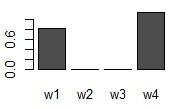
\includegraphics[width=\textwidth]{bilder/D14_II.png}
		\caption{Results for a nonobservable system with perturbation on knot $1$ and 
			parameter set II.} 
		\label{fig:notHIO_II}
	\end{minipage}

\end{figure}
	